\begin{center}
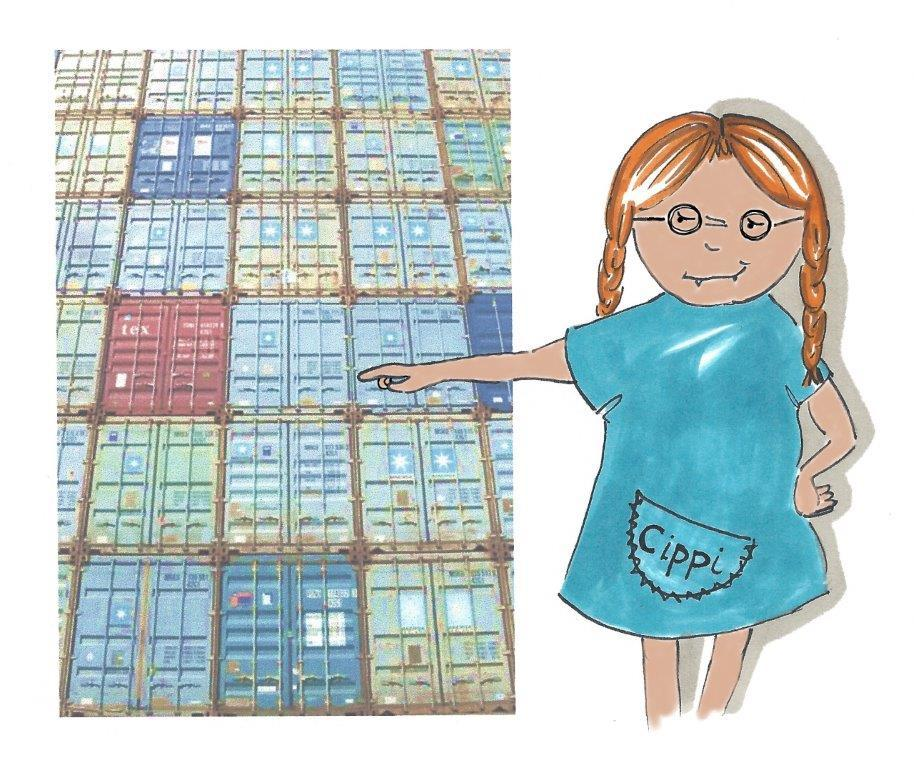
\includegraphics[width=0.6\textwidth]{content/3/chapter5/images/10.png}\\
Cippi inspects the container
\end{center}

C++20 has many improvements regarding containers of the Standard Template Library. First of all, std::vector and std::string have constexpr constructors and so can be used at compile time. All containers support consistent container erasure and the associative containers a member function contains. Additionally, std::string allows you to check for a prefix or suffix.

\subsubsubsection{5.3.1\hspace{0.2cm} constexpr Containers and Algorithms}

C++20 supports the constexpr containers std::vector and std::string, where constexpr means that the member functions of both containers can be applied at compile time. Additionally, the more than 100 \href{https://en.cppreference.com/w/cpp/algorithm}{algorithms} of the Standard Template Library are declared as constexpr.

Consequently, you can sort a std::vector of ints at compile time.

\hspace*{\fill} \\ %插入空行
\noindent
Sort a std::vector at compile time
\begin{lstlisting}[style=styleCXX]
// constexprVector.cpp

#include <algorithm>
#include <iostream>
#include <vector>

constexpr int maxElement() {
	std::vector myVec = {1, 2, 4, 3};
	std::sort(myVec.begin(), myVec.end());
	return myVec.back();
}
int main() {

	std::cout << '\n';
	
	constexpr int maxValue = maxElement();
	std::cout << "maxValue: " << maxValue << '\n';
	
	constexpr int maxValue2 = [] {
		std::vector myVec = {1, 2, 4, 3};
		std::sort(myVec.begin(), myVec.end()) ;
		return myVec.back();
	}();
	
	std::cout << "maxValue2: " << maxValue2 << '\n';
	
	std::cout << '\n';

}
\end{lstlisting}

The two containers std::vector (line 8 and 20) are sorted at compile time using constexpr-declared functions. In the first case, the function maxElement returns the last element of the vector myVec, which is its maximum value. In the second case, I use an immediately-invoked lambda that is declared constexpr.

\hspace*{\fill} \\ %插入空行
\begin{tcblisting}{breakable,commandshell={}}
maxValue: 4
maxValue2: 4
\end{tcblisting}

\begin{center}
Sort a std::vector at compile time
\end{center}

\subsubsubsection{5.3.2\hspace{0.2cm} std::array}

C++20 offers two convenient ways to create arrays. std::to\_array creates a std::array and std::make\_shared allows it to create a std::shared\_ptr of arrays.

\hspace*{\fill} \\ %插入空行
\noindent
5.3.2.1\hspace{0.2cm} std::to\_array

std::to\_array creates a std::array from an existing one-dimensional array. The elements of the created std::array are copy-initialized from the existing one-dimensional array.

The one-dimensional existing array can be a C-string, a std::initializer\_list, or a one-dimensional array of std::pair. The following example is from \href{https://en.cppreference.com/w/cpp/container/array/to_array}{cppreference.com/to\_array}.

\noindent
Create a std::array from various one-dimensional arrays
\begin{lstlisting}[style=styleCXX]
// toArray.cpp

#include <iostream>
#include <utility>
#include <array>
#include <memory>

int main() {

	std::cout << '\n';
	
	auto arr1 = std::to_array("A simple test");
	for (auto a: arr1) std::cout << a;
	std::cout << "\n\n";
	
	auto arr2 = std::to_array({1, 2, 3, 4, 5});
	for (auto a: arr2) std::cout << a;
	std::cout << "\n\n";
	
	auto arr3 = std::to_array<double>({0, 1, 3});
	for (auto a: arr3) std::cout << a;
	std::cout << '\n';
	std::cout << "typeid(arr3[0]).name(): " << typeid(arr3[0]).name() << '\n';
	std::cout << '\n';
	
	auto arr4 = std::to_array<std::pair<int, double>>({ {1, 0.0}, {2, 5.1},
	{3, 5.1} });
	for (auto p: arr4) {
		std::cout << "(" << p.first << ", " << p.second << ")" << '\n';
	}
	
	std::cout << "\n\n";

}
\end{lstlisting}

I created a std::array from a C-string (line 12), from a std::initializer\_list (lines 16 and 20), and from a std::initializer\_list of std::pair’s (line 26). In general, the compiler can deduce the type of the std::array. Optionally, you can specify the type (lines 20 and 26).

\begin{tcblisting}{breakable,commandshell={}}
A simple test

12345

013

typeid(arr3[0]).name(): d

(1, 0)
(2, 5.1)
(3, 5.1)
\end{tcblisting}

\begin{center}
Create various std::array from existing one-dimensional arrays
\end{center}

\hspace*{\fill} \\ %插入空行
\noindent
5.3.2.2\hspace{0.2cm} std::make\_shared

Since C++11, C++ supports the creation of the std::shared\_ptr via the factory function \href{https://en.cppreference.com/w/cpp/memory/shared_ptr/make_shared}{std::make\_shared}. With C++20, this factory function supports the creation of arrays of std::shared\_ptr.

\begin{itemize}
\item 
std::shared\_ptr<double[]> shar = std::make\_shared<double[]>(1024): creates a shared\_ptr with 1024 default-initialized doubles

\item 
std::shared\_ptr<double[]> shar = std::make\_shared<double[]>(1024, 1.0): creates a shared\_ptr with 1024 doubles initialized to 1.0
\end{itemize}

\subsubsubsection{5.3.3\hspace{0.2cm} Consistent Container Erasure}

Before C++20, removing elements from a container was too complicated. Let me show why.

\noindent
5.3.3.1\hspace{0.2cm} The erase-remove Idiom

Removing an element from a container seems to be quite easy. In the case of a std::vector, you can use the function std::remove\_if.

\noindent
Using std::remove\_if to remove elements from a container
\begin{lstlisting}[style=styleCXX]
// removeElements.cpp

#include <algorithm>
#include <iostream>
#include <vector>

int main() {

	std::cout << '\n';
	
	std::vector myVec{-2, 3, -5, 10, 3, 0, -5 };
	
	for (auto ele: myVec) std::cout << ele << " ";
	std::cout << "\n\n";
	
	std::remove_if(myVec.begin(), myVec.end(), [](int ele){ return ele < 0; });
	for (auto ele: myVec) std::cout << ele << " ";
	
	std::cout << "\n\n";

}
\end{lstlisting}

The program removeElements.cpp removes all elements from the std::vector that are less than zero. Easy, right? Maybe not; now, you fall into the trap that is well-known to many seasoned C++ programmer.

\begin{center}
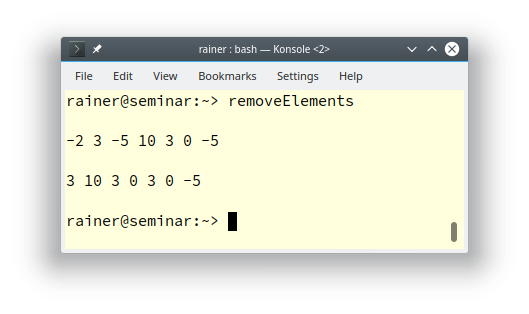
\includegraphics[width=0.6\textwidth]{content/3/chapter5/images/11.png}\\
Using std::remove\_if to remove elements from a container
\end{center}

std::remove\_if (lines 16) does not remove anything. The std::vector still has the same number of arguments. Both algorithms return the new logical end of the modified container.

To modify a container, you have to apply the new logical end to the container.

\noindent
Applying the erase-remove idiom to a container
\begin{lstlisting}[style=styleCXX]
// eraseRemoveElements.cpp

#include <algorithm>
#include <iostream>
#include <vector>

int main() {
	
	std::cout << '\n';
	
	std::vector myVec{-2, 3, -5, 10, 3, 0, -5 };
	
	for (auto ele: myVec) std::cout << ele << " ";
	std::cout << "\n\n";
	
	auto newEnd = std::remove_if(myVec.begin(), myVec.end(),
	[](int ele){ return ele < 0; });
	myVec.erase(newEnd, myVec.end());
	// myVec.erase(std::remove_if(myVec.begin(), myVec.end(),
	//              [](int ele){ return ele < 0; }), myVec.end());
	for (auto ele: myVec) std::cout << ele << " ";
	
	std::cout << "\n\n";

}
\end{lstlisting}

Line (16) returns the new logical end newEnd of the container myVec. This new logical end is applied in line 18 to remove all elements from myVec starting at newEnd. When you apply the functions remove and erase in one expression such as in line 19, you see exactly why this construct is called erase-remove idiom.

\begin{center}
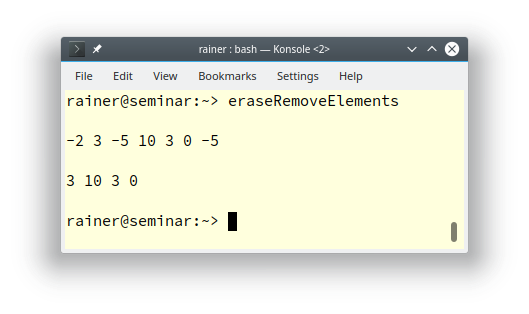
\includegraphics[width=0.6\textwidth]{content/3/chapter5/images/12.png}\\
Using the erase-remove idiom
\end{center}

Thanks to the new functions erase and erase\_if in C++20, erasing elements from containers is far more convenient.

\noindent
5.3.3.2\hspace{0.2cm}  erase and erase\_if in C++20

With erase and erase\_if, you can directly operate on the container. In contrast, the previously presented erase-remove idiom is quite verbose: it requires two iterations.

Let’s see what the new functions erase and erase\_if mean in practice. The following program erases elements from a few containers.

\noindent
Erase elements from a container
\begin{lstlisting}[style=styleCXX]
// eraseCpp20.cpp

#include <iostream>
#include <numeric>
#include <deque>
#include <list>
#include <string>
#include <vector>

template <typename Cont>
void eraseVal(Cont& cont, int val) {
	std::erase(cont, val);
}

template <typename Cont, typename Pred>
void erasePredicate(Cont& cont, Pred pred) {
	std::erase_if(cont, pred);
}

template <typename Cont>
void printContainer(Cont& cont) {
	for (auto c: cont) std::cout << c << " ";
	std::cout << '\n';
}

template <typename Cont>
void doAll(Cont& cont) {
	printContainer(cont);
	eraseVal(cont, 5);
	printContainer(cont);
	erasePredicate(cont, [](auto i) { return i >= 3; } );
	printContainer(cont);
}

int main() {

	std::cout << '\n';
	
	std::string str{"A Sentence with an E."};
	std::cout << "str: " << str << '\n';
	std::erase(str, 'e');
	std::cout << "str: " << str << '\n';
	std::erase_if( str, [](char c){ return std::isupper(c); });
	std::cout << "str: " << str << '\n';
	
	std::cout << "\nstd::vector " << '\n';
	std::vector vec{1, 2, 3, 4, 5, 6, 7, 8, 9};
	doAll(vec);
	
	std::cout << "\nstd::deque " << '\n';
	std::deque deq{1, 2, 3, 4, 5, 6, 7, 8, 9};
	doAll(deq);
	
	std::cout << "\nstd::list" << '\n';
	std::list lst{1, 2, 3, 4, 5, 6, 7, 8, 9};
	doAll(lst);

}
\end{lstlisting}

Line 41 erases all the 'e' characters from the given string str. Line 43 applies the lambda expression to the same string and erases all the upper case letters.

In the rest of the program, elements of the sequence containers std::vector (line 47), std::deque (line 51), and std::list (line 55) are erased. On each container, the function template doAll (line 26) is applied. doAll erases the element 5 and all elements greater than or equal to 3. The function template eraseVal (line 10) uses the new function erase and the function template erasePredicate (line 15) uses the new function erase\_if.

\begin{center}
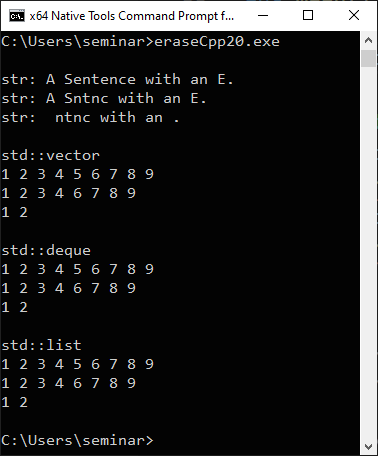
\includegraphics[width=0.6\textwidth]{content/3/chapter5/images/13.png}\\
Application of the new functions erase and erase\_if
\end{center}

The new functions erase and erase\_if can be applied to all containers of the Standard Template Library. This does not hold for the next convenience function contains, which requires an associative container.

\subsubsubsection{5.3.4\hspace{0.2cm} contains for Associative Containers}

Thanks to the function contains, you can easily check if an element exists in an associative container.
Stop, you may say, we can already do this with find or count.

No, both functions are not beginner-friendly and have their downsides.

\noindent
Erase elements from a container
\begin{lstlisting}[style=styleCXX]
// checkExistence.cpp

#include <set>
#include <iostream>

int main() {

	std::cout << '\n';
	
	std::set mySet{3, 2, 1};
	if (mySet.find(2) != mySet.end()) {
		std::cout << "2 inside" << '\n';
	}
	
	std::multiset myMultiSet{3, 2, 1, 2};
	if (myMultiSet.count(2)) {
		std::cout << "2 inside" << '\n';
	}
	
	std::cout << '\n';

}
\end{lstlisting}

The functions produce the expected result.

\begin{tcblisting}{breakable,commandshell={}}
2 inside
2 inside
\end{tcblisting}

\begin{center}
Use of find and count to check if a container has a given element
\end{center}

There are issues with both calls. The find call (line 11) is too verbose. The same argument holds for the count call (line 16). The count call also has a performance issue. When you want to know if an element is in a container, you should stop when you found it and not count until the end. In the concrete case myMultiSet.count(2) returned 2.

Unlike find and count, the contains member function in C++20 is quite convenient to use.

\noindent
contains in C++20
\begin{lstlisting}[style=styleCXX]
// containsElement.cpp

#include <iostream>
#include <set>
#include <map>
#include <unordered_set>
#include <unordered_map>

template <typename AssocCont>
bool containsElement5(const AssocCont& assocCont) {
	return assocCont.contains(5);
}

int main() {

	std::cout << std::boolalpha;
	
	std::cout << '\n';
	
	std::set<int> mySet{1, 2, 3, 4, 5, 6, 7, 8, 9, 10};
	std::cout << "containsElement5(mySet): " << containsElement5(mySet);
	
	std::cout << '\n';
	
	std::unordered_set<int> myUnordSet{1, 2, 3, 4, 5, 6, 7, 8, 9, 10};
	std::cout << "containsElement5(myUnordSet): " << containsElement5(myUnordSet);
	
	std::cout << '\n';
	
	std::map<int, std::string> myMap{ {1, "red"}, {2, "blue"}, {3, "green"} };
	std::cout << "containsElement5(myMap): " << containsElement5(myMap);
	
	std::cout << '\n';
	
	std::unordered_map<int, std::string> myUnordMap{ {1, "red"},
	                                                 {2, "blue"}, {3, "green"} };
	std::cout << "containsElement5(myUnordMap): " << containsElement5(myUnordMap);
	
	std::cout << '\n';

}
\end{lstlisting}

There is not much to add to this example. The function template containsElement5 returns true if the associative container contains the key 5. In my example, I used only the associative containers std::set, std::unordered\_set, std::map, and std::unordered\_set, none of which can hold a given key more than once.

\begin{center}
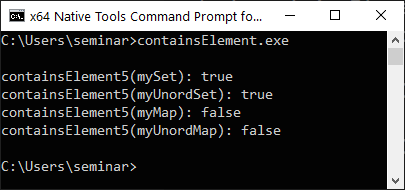
\includegraphics[width=0.6\textwidth]{content/3/chapter5/images/14.png}\\
Use of the new function contains
\end{center}

\subsubsubsection{5.3.5\hspace{0.2cm} String prefix and suffix checking}

std::string gets new member functions starts\_with and ends\_with. They allow you to check if a std::string starts or ends with a specified substring.

\noindent
Check if a string starts with or ends with a given string
\begin{lstlisting}[style=styleCXX]
// stringStartsWithEndsWith.cpp

#include <iostream>
#include <string_view>
#include <string>

template <typename PrefixType>
void startsWith(const std::string& str, PrefixType prefix) {
	std::cout << " starts with " << prefix << ": "
			  << str.starts_with(prefix) << '\n';
}

template <typename SuffixType>
void endsWith(const std::string& str, SuffixType suffix) {
	std::cout << " ends with " << suffix << ": "
			  << str.ends_with(suffix) << '\n';
}

int main() {

	std::cout << '\n';
	
	std::cout << std::boolalpha;
	
	std::string helloWorld("Hello World");
	
	std::cout << helloWorld << '\n';
	
	startsWith(helloWorld, helloWorld);
	
	startsWith(helloWorld, std::string_view("Hello"));
	
	startsWith(helloWorld, 'H');
	
	std::cout << "\n\n";
	
	std::cout << helloWorld << '\n';
	
	endsWith(helloWorld, helloWorld);
	
	endsWith(helloWorld, std::string_view("World"));
	
	endsWith(helloWorld, 'd');

}
\end{lstlisting}

Both member functions starts\_with and ends\_with are predicates and, hence, return a boolean. You can invoke the new member functions starts\_with and ends\_with with a std::string (lines 29 and 39), a std::string\_view (lines 31 and 41), and a char (lines 33 and 43).

\begin{tcblisting}{breakable,commandshell={}}
Hello World
            starts with Hello World: true
            starts with Hello: true
            starts with H: true
            
Hello World
            ends with Hello World: true
            ends with World: true
            ends with d: true
\end{tcblisting}

\begin{center}
Check if a string starts with or ends with a given string
\end{center}

\begin{tcolorbox}[breakable,enhanced jigsaw,colback=mygreen!5!white,colframe=mygreen!75!black,title={Distilled Information}]
	
\begin{itemize}
\item 
std::vector and std::string have constexpr constructors and can, therefore, be instantiated at compile time. Thanks to the constexpr algorithms of the Standard Template Library (STL), you can manipulate them at compile time.

\item 
C++20 offers two convenient ways to create arrays. std::to\_array creates a std::array and std::make\_shared allows the creation of a std::shared\_ptr wrapping a C-array.

\item 
The new algorithm std::erase and std::erase\_if are used to erase specific elements (erase) or elements satisfying a predicate (erase\_if) from an arbitrary container of the STL.

\item 
Thanks to the member function contains, you can check for an associative container if it has the requested key.

\item 
std::string supports the new member function start\_with and end\_with to check if the container has a specific prefix or suffix.
\end{itemize}
	
\end{tcolorbox}


\newpage


















